\chapter{张量范畴与弦网模型}

\section{范畴论基础}

\emph{范畴论} (category theory) 用以抽象地刻画一些数学结构之间的关系,它主要描述了“对象”之间的作用,即\emph{映射} (mapping)。拓扑序理论中所研究的,正是带有了某些附加结构的范畴。

一个\emph{范畴} $\mathcal{C}$ 由其中的\emph{对象} (object) $x\in\mathcal{C}$ 和这些对象之间的\emph{态射} (morphism) $f\colon x\to y$ 组成。对象之间的态射满足以下三个条件:
\begin{itemize}
  \item \emph{复合性} (composition):对于范畴 $\mathcal{C}$ 中的对象 $x$、$y$、$z$,若 $f\colon x\to y$ 和 $g\colon y\to z$ 为态射,则存在复合态射 $g\circ f\colon x\to z$;
  \item \emph{结合律} (associativity):若 $\mathcal{C}$ 中有态射 $f\colon x\to y$、$g\colon y\to z$、$h\colon z\to w$,则有
    \begin{equation}
      (h\circ g)\circ f = h\circ (g\circ f);
    \end{equation}
  \item \emph{单位元} (identity):对于 $\forall x\in\mathcal{C}$,都存在恒等态射 $\id_x\colon x\to x$,使得
    \begin{equation}
      f \circ \id_x = \id_x \circ f = f, \quad \forall f\colon x\to y.
    \end{equation}
\end{itemize}
态射也可记为 $f\in\Hom_{\mathcal{C}}(x,y)$,其中 $\Hom_{\mathcal{C}}(x,y)$ 称为同态集 (hom-set)。如果 $x=y$,则称 $f$ 为\emph{自同态} (endomorphism),记为 $f\in\End_{\mathcal{C}}(x)$。

\emph{函子} (functor) 是范畴之间保结构的映射。具体而言,对于范畴 $\mathcal{C}$、$\mathcal{D}$,函子 $F\colon\mathcal{C}\to\mathcal{D}$ 会将 $\mathcal{C}$ 中的对象 $x$ 映射到 $\mathcal{D}$ 中的对象 $F(x)$,而将 $\mathcal{C}$ 中的态射 $f\colon x\to y$ 映射到 $\mathcal{D}$ 中的态射 $F_f\colon F(x)\to F(y)$,并且保持复合性与单位元的成立,即
\begin{align}
  F_{\id_x} &= \id_{F(x)} \colon F(x) \to F(x), \quad \forall x\in\mathcal{C}, \\
  F_{g\circ f} &= F_g \circ F_f \colon F(x) \to F(z), \quad \forall f\colon x\to y, \, g\colon y\to z.
\end{align}

在函子之上可进一步定义\emph{自然变换} (natural transformation)。对于两个函子 $F\colon\mathcal{C}\to\mathcal{D}$ 和 $G\colon\mathcal{C}\to\mathcal{D}$,自然变换 $\tau\colon F\Rightarrow G$ 由其分量 $\tau_x$(这是范畴 $\mathcal{D}$ 中的一个态射)定义:
\begin{equation}
  \tau_x\colon F(x)\to G(x), \quad \forall x\in\mathcal{C},
\end{equation}
它满足
\begin{equation}
  \tau_y \circ F_f = G_f \circ \tau_x, \quad \forall f\colon x\to y.
\end{equation}
如图~\ref{fig:natural-transformation},自然变换可以用交换图来直观地表示。若 $\tau$ 的每一分量 $\tau_x$ 均可逆(即存在 $\tau_x^{-1}$ 使得 $\tau^{-1}_x\circ\tau_x=\id_{F(x)}$ 且 $\tau_x\circ\tau^{-1}_x = \id_{G(x)}$),则称其为\emph{自然同构} (natural isomorphism),我们用 $\similarrightarrow$ 来表示。

\begin{figure}[htb]
  \centering
  \begin{tabular}{c@{\qquad}c}
    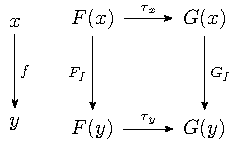
\includegraphics{images/natural-transformation-1.pdf} &
    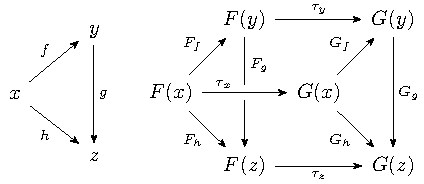
\includegraphics{images/natural-transformation-2.pdf} \\
    (a) & (b)
  \end{tabular}
  \caption[自然变换对应的交换图]{自然变换对应的交换图。(a) 此图是“可交换的”,即从 $F(x)$ 到 $G(y)$ 的两条路径等价;(b) 对于结合律的“提升”,图中三棱柱的三个侧面都是可交换的。}
  \label{fig:natural-transformation}
\end{figure}

\begin{example}
  对于任意的交换环 $K$,以其中元素构成的 $n\times n$ 的非奇异矩阵组成了一般线性群 $GL_n(K)$。对于环同态 $f\colon K\to L$,显然可以构建群同态 $GL_n f\colon GL_n(K)\to GL_n(L)$。因此,$GL_n$ 即为交换环范畴 $\mathbf{CRng}$ 到群范畴 $\mathbf{Grp}$ 的函子。

  设非奇异矩阵 $M\in GL_n(K)$,则其行列式 $\det_K(M)$ 为 $K$ 中的可逆元(即单位),因而 $\det_K$ 是群同态 $GL_n(K)\to K^\times$,其中 $K^\times$ 为 $K$ 的可逆元群。另一方面,当把环同态 $f$ 限制在可逆元群上时,可得群同态 $f^\times\colon K^\times\to L^\times$,因而 $(\cdot)^\times$ 同样也是 $\mathbf{CRng}$ 到 $\mathbf{Grp}$ 的函子。根据定义,$\det\colon GL_n\Rightarrow(\cdot)^\times$ 即为自然变换,它满足 $\det_L\circ\,GL_n f=f^\times\circ \det_K$。
\end{example}

% \begin{example}
%   在 Haskell 编程语言中,类型为范畴 $\mathbf{Hask}$ 中的对象,而纯函数为态射。函子可由类型类 (type class) 来定义,例如 \verb|List| 可以将类型 \verb|T| 构造为对应的数组 \verb|[T]|,并且通过 \verb|fmap| 将以 \verb|T| 类型为参数的纯函数转换为以 \verb|[T]| 类型为参数的纯函数。自然变换则由参数多态 (parametric polymorphism) 实现。例如,一个安全的(不引发异常)返回数组首元素的函数可按下面的方式定义:
% \begin{verbatim}
%   head :: [T] -> Maybe T
%   head []     = Nothing
%   head (x:xs) = Just x
% \end{verbatim}
%   因此 \verb|head| 函数是从 \verb|List| 到 \verb|Maybe| 的自然变换。
% \end{example}

\emph{弦图} (string diagram) 可以更直观地描述范畴的概念。其中,带箭头的直线或曲线代表对象,盒子代表态射:
\begin{equation}
  f\colon x\to y \quad \coloneq \quad
  \begin{tikzpicture}[baseline=1cm]
  \draw [->-=0.2, ->-=0.8]
    (0,2) node [above] {$x$} -- (0,0) node [below] {$y$}
    (0,1) node [draw, fill=white, anchor=base] {$\scriptstyle f$};
\end{tikzpicture}
 \, .
\end{equation}
这样态射的复合就可以表示为连在一起的两个盒子:
\begin{equation}
  \begin{tikzpicture}[baseline=1cm]
  \draw [->-=0.2, ->-=0.9] (0,2) node [above] {$x$} -- (0,0) node [below] {$z$};
  \draw (0,1) node [draw, fill=white, anchor=base] {$\scriptstyle g\circ f$};
  \draw (1,1) node [anchor=base] {=};
  \draw [->-=0.53] (2,2) node [above] {$x$} -- (2,0) node [below] {$z$};
  \draw (2,1.5) node [draw, fill=white, anchor=base, minimum size=0.45cm] {$\scriptstyle f$}
        (2,0.5) node [draw, fill=white, anchor=base, minimum size=0.45cm] {$\scriptstyle g$}
        (2.35,1) node {$y$};
\end{tikzpicture}
.
\end{equation}

\section{张量范畴与融合范畴}

\subsection{张量范畴}

我们可以在范畴中引入一些结构,使其具有新的特性。引入了张量积的范畴为\emph{张量范畴} (tensor category)。它最基本也最重要的例子是向量空间(或对应的范畴 $\mathbf{Vec}$),其中的张量积结构即为两个向量空间和相应线性变换的直积。一个张量范畴 $\mathcal{C}$ 由下面的条件定义:
\begin{itemize}
  \item \emph{张量积} (tensor product) $\otimes\colon\mathcal{C}\times\mathcal{C}\to\mathcal{C}$ 和\emph{单位对象} (unit object) $\1\in\mathcal{C}$;
  \item \emph{结合子} (associator) $\alpha$,它是一个自然同构:
    \begin{equation}
      \alpha_{x,y,z} \colon (x\otimes y)\otimes z \similarrightarrow x\otimes(y\otimes z), \quad \forall x,y,z \in \mathcal{C};
    \end{equation}
  \item \emph{左右单位子} (left/right unitor),同样也是自然同构:
    \begin{equation}
      \lambda_x \colon \1\otimes x \similarrightarrow x, \quad
      \rho_x    \colon x\otimes\1  \similarrightarrow x, \quad
      \forall x \in \mathcal{C}.
    \end{equation}
\end{itemize}
它们需要满足五边形方程和三角形方程(图~\ref{fig:pentagon-triangle-equation})。

\begin{figure}[htb]
  \centering
  \begin{tabular}{cc}
    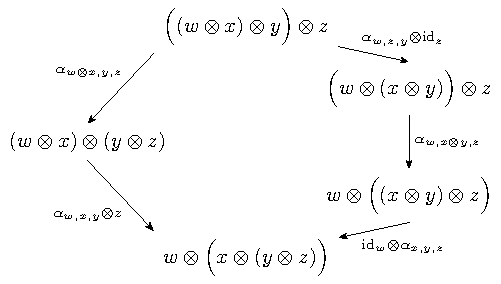
\includegraphics{images/pentagon-equation.pdf} &
    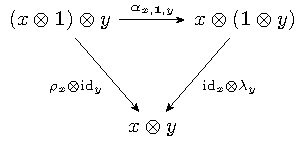
\includegraphics{images/triangle-equation.pdf} \\
    (a) & (b)
  \end{tabular}
  \caption[五边形方程和三角形方程对应的交换图]{五边形方程 (a) 和三角形方程 (b) 对应的交换图。}
  \label{fig:pentagon-triangle-equation}
\end{figure}

如果上述定义中的 $\similarrightarrow$ 可以取为等号,则称该张量范畴是\emph{严格} (strict) 的,此时 $\alpha$、$\lambda$ 和 $\rho$ 均为恒等变换。根据 MacLane \emph{一致性定理} (coherence theorem),每个张量范畴都等价于一个严格张量范畴。因此我们之后可以只考虑严格张量范畴的情况。此时张量积表达式中的括号和单位对象都可以忽略。

一个张量范畴也是一个\emph{幺半群} (monoid),因为范畴的单位对象可以作为群的单位元,而张量积可以作为群乘法。所以张量范畴也被称为\emph{幺半范畴} (monoidal category)。

\subsection{对偶}

类似于对偶空间的概念,我们可以在张量范畴中引入\emph{对偶} (dual) 的概念。$x\in\mathcal{C}$ 的\emph{右对偶} (right dual) $x^\vee$ 通过以下两个态射定义:
\begin{equation}
  e_x\colon x^\vee\otimes x\to\1, \quad i_x\colon\1\to x\otimes x^\vee,
\end{equation}
它们需要满足\emph{刚性公理} (rigidity axioms):
\begin{equation}
  \begin{aligned}
    (\id_x\otimes e_x) \circ (i_x\otimes\id_x) &= \id_x, \\
    (e_x\otimes\id_{x^\vee}) \circ (\id_{x^\vee}\otimes i_x) &= \id_{x^\vee}.
  \end{aligned}
\end{equation}
如果在弦图中省略单位元(对应于物理中的真空态),则 $e_x$ 和 $i_x$ 可以表示为
\begin{equation}
  \begin{tikzpicture}[baseline=1cm]
  \draw [->-={1/7}, ->-={10/21}, ->-=0.9]
    (0  ,2) node [above=4pt, anchor=base] {$x^*$} -- ++ (0,-1)
    (0.8,2) node [above=4pt, anchor=base] {$x$}   -- ++ (0,-1)
    (0.4,1) -- ++ (0,-1) node [below] {$\mathbf{1}$};
  \draw (0.4,1) node [draw, minimum width=1.2cm, minimum height=0.5cm, fill=white, anchor=base] {$e_x$};
  \draw (1.4,1.03) node {=};
  \draw [->-=0.74] (2,1) -- ++ (0,1) node [above=4pt, anchor=base] {$x$};
  \draw [->-=0.44] (2.8,2) node [above=4pt, anchor=base] {$x$} -- ++ (0,-1);
  \draw (2.4,1) node [draw, minimum width=1.2cm, minimum height=0.5cm, fill=white, anchor=base] {$e_x$};
  \draw (3.4,1.03) node {=};
  \draw [->-=0.92] (4.7,2) node [above=4pt, anchor=base] {$x$}
    -- (4.7,1) .. controls (4.7,0.9) and (4.7,0.4) .. (4.3,0.4)
               .. controls (3.9,0.4) and (3.9,0.9) .. (3.9,1  ) -- (3.9,2);
\end{tikzpicture}
,
  \qquad
  \begin{tikzpicture}[baseline=1cm]
  \draw [->-={1/7}, ->-=0.567, ->-=0.9]
    (0.4,2) node [above=4pt, anchor=base] {$\mathbf{1}$} -- ++ (0,-1)
    (0  ,1) -- ++ (0,-1) node [below=10pt, anchor=base] {$x$}
    (0.8,1) -- ++ (0,-1) node [below=10pt, anchor=base] {$x^*$};
  \draw (0.4,1) node [draw, minimum width=1.2cm, minimum height=0.5cm, fill=white, anchor=base] {$i_x$};
  \draw (1.4,1.03) node {=};
  \draw [->-=0.72] (2  ,1) -- ++ (0,-1) node [below=10pt, anchor=base] {$x$};
  \draw [->-=0.46] (2.8,0) node [below=10pt, anchor=base] {$x$} -- ++ (0,1);
  \draw (2.4,1) node [draw, minimum width=1.2cm, minimum height=0.5cm, fill=white, anchor=base] {$i_x$};
  \draw (3.4,1.03) node {=};
  \draw [->-=0.92] (4.7,0) node [below=10pt, anchor=base] {$x$}
    -- (4.7,1) .. controls (4.7,1.1) and (4.7,1.6) .. (4.3,1.6)
               .. controls (3.9,1.6) and (3.9,1.1) .. (3.9,1  ) -- (3.9,0);
\end{tikzpicture}
.
\end{equation}
这可以类比于量子力学中的湮灭与产生算符。(右对偶的)刚性公理则可表示为
\begin{equation}
  \begin{tikzpicture}[baseline=0.8cm]
  \draw [->-=0.87] (1.2,1.6) node [above] {$x$}
    -- (1.2,0.5)
    .. controls (1.2,0.4) and (1.2,0.0) .. (0.9,0.0)
    .. controls (0.6,0.0) and (0.6,0.4) .. (0.6,0.5)
    -- (0.6,1.1)
    .. controls (0.6,1.2) and (0.6,1.6) .. (0.3,1.6)
    .. controls (0.0,1.6) and (0.0,1.2) .. (0.0,1.1)
    -- (0.0,0.0);
  \draw (1.8,0.8) node {=};
  \draw [->-=0.55] (2.4,1.6) node [above] {$x$} -- (2.4,0);
\end{tikzpicture}
,
  \qquad
  \begin{tikzpicture}[baseline=0.8cm]
  \draw [->-=0.87] (1.2,0.0) node [below] {$x$}
    -- (1.2,1.1)
    .. controls (1.2,1.2) and (1.2,1.6) .. (0.9,1.6)
    .. controls (0.6,1.6) and (0.6,1.2) .. (0.6,1.1)
    -- (0.6,0.5)
    .. controls (0.6,0.4) and (0.6,0.0) .. (0.3,0.0)
    .. controls (0.0,0.0) and (0.0,0.4) .. (0.0,0.5)
    -- (0.0,1.6);
  \draw (1.8,0.8) node {=};
  \draw [->-=0.57] (2.4,0) node [below] {$x$} -- (2.4,1.6);
\end{tikzpicture}
.
\end{equation}

同理,我们还可以定义\emph{左对偶} (left dual):
\begin{equation}
  e'_x \colon x\otimes \ldual{x}\to\1, \quad i'_x\colon \1\to\ldual{x}\otimes x.
  \label{eq:left-dual}
\end{equation}
这实际上只需要对上面的图沿水平方向做一下镜像操作。如果 $\mathcal{C}$ 中的每个对象既有左对偶也有右对偶,则称其为是\emph{刚性} (rigid) 的或\emph{自治} (autonomous) 的;而如果 $\forall x\in\mathcal{C}$,都有 $x=x^\vee$,则称 $\mathcal{C}$ 是\emph{自对偶} (self-dual) 的。

\subsection{中枢与球状结构}

我们知道有限维向量空间 $V$ 的二重对偶 $V^{\vee\vee}$ 同构于 $V$。这在张量范畴中的推广即为\emph{中枢} (pivotal) 结构,它是由以下的自然同构给出的:
\begin{equation}
  \delta_x \colon x \similarrightarrow x^{\vee\vee}, \quad \forall x\in\mathcal{C},
\end{equation}
且需满足
\begin{equation}
  \delta_{x\otimes y} = \delta_x\otimes\delta_y, \quad
  \delta_\1 = \id_\1, \quad
  \delta_{x^\vee} = (\delta_x^\vee)^{-1}.
\end{equation}
根据右对偶的定义,可有
\begin{equation}
  e_x\colon x^\vee\otimes x \similarrightarrow x^\vee\otimes x^{\vee\vee}\to\1, \quad
  i_x\colon \1\to x\otimes x^\vee \similarrightarrow x^{\vee\vee}\otimes x^\vee.
\end{equation}
对比式~\eqref{eq:left-dual},可以发现 $x^{\vee\vee}$ 也是 $x^\vee$ 的左对偶。若令 $y=x^\vee$,即有 $\ldual{y}=y^\vee$,也就是说在中枢范畴中可以不再区分左右对偶。

对于中枢范畴 $\mathcal{C}$ 中的自同态 $f\in\End_{\mathcal{C}}(x)$,可以定义\emph{左右迹} (left/right trace):
\begin{equation}
  \begin{aligned}
    \tr_{\text{L}} f &\colon \1 \xrightarrow{i_{x^\vee}} x^\vee\otimes x^{\vee\vee}
                                \xrightarrow{\id_{x^\vee}\otimes\delta_x^{-1}} x^\vee\otimes x
                                \xrightarrow{\id_{x^\vee}\otimes f} x^\vee\otimes x
                                \xrightarrow{e_x} \1, \\
    \tr_{\text{R}} f &\colon \1 \xrightarrow{i_x} x\otimes x^\vee
                                \xrightarrow{f\otimes\id_{x^\vee}} x\otimes x^\vee
                                \xrightarrow{\delta_x\otimes\id_{x^\vee}} x^{\vee\vee}\otimes x^\vee
                                \xrightarrow{e_{x^\vee}} \1.
  \end{aligned}
\end{equation}
当 $f=\id_x$ 时,还可以定义\emph{左右维数} (left/right dimension):
\begin{equation}
  \dim_{\text{L}} x \coloneq \tr_{\text{L}}\id_x, \quad
  \dim_{\text{R}} x \coloneq \tr_{\text{R}}\id_x.
  \label{eq:left-right-dimension}
\end{equation}
迹和维数可以用下图来描述:
\begin{equation}
  \tr_{\text{L}}  f = \begin{tikzpicture}[baseline=1.05cm]
  \draw [->-=0.27]
      (0.5,0.0)
    .. controls (0.0,0.0) and (0.0,0.5) .. (0.0,0.8)
    -- (0.0,1.4)
    .. controls (0.0,1.7) and (0.0,2.2) .. (0.5,2.2)
    .. controls (1.0,2.2) and (1.0,1.7) .. (1.0,1.4)
    -- (1.0,0.8)
    .. controls (1.0,0.5) and (1.0,0.0) .. cycle
    (1.0,0.0) node {$x$}
    (1.0,1.05) node [draw, fill=white, anchor=base] {$f$};
\end{tikzpicture}
 \, , \quad
  \tr_{\text{R}}  f = \begin{tikzpicture}[baseline=1.05cm]
  \draw [->-=0.27]
      (0.5,0.0)
    .. controls (1.0,0.0) and (1.0,0.5) .. (1.0,0.8)
    -- (1.0,1.4)
    .. controls (1.0,1.7) and (1.0,2.2) .. (0.5,2.2)
    .. controls (0.0,2.2) and (0.0,1.7) .. (0.0,1.4)
    -- (0.0,0.8)
    .. controls (0.0,0.5) and (0.0,0.0) .. cycle
    (1.0,0.0) node {$x$}
    (1.0,1.05) node [draw, fill=white, anchor=base] {$f$};
\end{tikzpicture}
 \, ; \quad
  \dim_{\text{L}} x = \begin{tikzpicture}[baseline=1.05cm]
  \draw [->-=0.27]
      (0.5,0.0)
    .. controls (0.0,0.0) and (0.0,0.5) .. (0.0,0.8)
    -- (0.0,1.4)
    .. controls (0.0,1.7) and (0.0,2.2) .. (0.5,2.2)
    .. controls (1.0,2.2) and (1.0,1.7) .. (1.0,1.4)
    -- (1.0,0.8)
    .. controls (1.0,0.5) and (1.0,0.0) .. cycle
    (1.0,0.0) node {$x$};
\end{tikzpicture}
 \!, \quad
  \dim_{\text{R}} x = \begin{tikzpicture}[baseline=1.05cm]
  \draw [->-=0.27]
      (0.5,0.0)
    .. controls (1.0,0.0) and (1.0,0.5) .. (1.0,0.8)
    -- (1.0,1.4)
    .. controls (1.0,1.7) and (1.0,2.2) .. (0.5,2.2)
    .. controls (0.0,2.2) and (0.0,1.7) .. (0.0,1.4)
    -- (0.0,0.8)
    .. controls (0.0,0.5) and (0.0,0.0) .. cycle
    (1.0,0.0) node {$x$};
\end{tikzpicture}
 \!.
\end{equation}
如果对于任意的 $f\in\End_{\mathcal{C}}(x)$ 都有 $\tr_{\text{L}}f=\tr_{\text{R}}f$,则称 $\mathcal{C}$ 是\emph{球状} (spherical) 的。

\subsection{融合范畴}

范畴中还可以引入\emph{直和} (direct sum) 的结构。若范畴 $\mathcal{C}$ 中的对象均可分解为\emph{简单对象} (simple object) 的直和:
\begin{equation}
  x = \bigoplus_{i\in I} n_i x_i, \quad \forall x \in \mathcal{C},
\end{equation}
其中 $x_i\in\mathcal{C}$ 是简单对象,$I$ 是非零简单对象的指标集,而系数 $n_i\in\mathbb{Z}_+$,则称 $\mathcal{C}$ 是一个\emph{半单范畴} (semi-simple category)。简单对象的例子包括向量空间范畴 $\mathbf{Vec}$ 中的一维空间(直线),以及 Abel 群范畴 $\mathbf{Ab}$ 中的单群。

若张量范畴 $\mathcal{C}$ 同时也是半单的,并且简单对象只有有限多个,那么这样的 $\mathcal{C}$ 称为\emph{融合范畴} (fusion category)。此时简单对象的张量积可以写成:
\begin{equation}
  x_a \otimes x_b = \bigoplus_c N_{ab}^c x_c,
\end{equation}
其中 $N_{ab}^c\in\mathbb{Z}_+$,称为\emph{融合系数} (fusion coefficient)。在物理学中一般可以假设 $N_{ab}^c$ 只能取到 0 或 1,即是否允许该融合发生。所有允许的融合称为 \emph{融合规则} (fusion rule)。融合范畴还要与张量范畴的结构相容,这意味着
\begin{equation}
  N_{\1 a}^b = N_{a\1}^b = \delta_{ab}, \quad
  \sum_x N_{ax}^z N_{bc}^x = \sum_y N_{ab}^y N_{yc}^z.
\end{equation}
我们还要求融合范畴是刚性且自对偶的,此时可以证明
\begin{equation}
  N_{ab}^c = N_{ba}^c = N_{ac}^b = N_{ca}^b = N_{bc}^a = N_{cb}^a,
\end{equation}
即融合系数关于所有指标均对称。

定义矩阵 $(N_a)_{bc}\coloneq N_{ab}^c$,根据 Perron--Frobenius 定理,可知 $N_a$ 存在最大的非负特征值,这定义为简单对象 $a$ 的\emph{量子维数} (quantum dimension)或 Perron--Frobenius 维数。可以证明,量子维数与式~\eqref{eq:left-right-dimension} 中通过迹定义的维数是相同的。

融合的逆运算是\emph{拆分} (splitting)。简单对象的融合与拆分都可以用弦图来表示:
\begin{equation}
  \begin{tikzpicture}[baseline=0cm]
  \draw
    (0:0) -- (150:0.5) node [above] {$a$}
    (0:0) -- (30:0.5)  node [above] {$b$}
    (0:0) -- (-90:0.4) node [below] {$c$};
\end{tikzpicture}

  \in \Hom_{\mathcal{C}}(a\otimes b, c) \eqcolon V^{ab}_c, \quad
  \begin{tikzpicture}[baseline=0cm]
  \draw
    (0:0) -- (90:0.4)   node [above] {$c$}
    (0:0) -- (-150:0.5) node [below=0.4cm, anchor=base] {$a$}
    (0:0) -- (-30:0.5)  node [below=0.4cm, anchor=base] {$b$};
\end{tikzpicture}

  \in \Hom_{\mathcal{C}}(c, a\otimes b) \eqcolon V_{ab}^c.
\end{equation}
由于 $\mathcal{C}$ 的刚性和自对偶性,我们可以省略弦图中的箭头。此时,$\Hom_{\mathcal{C}}(a\otimes b,c)$ 和 $\Hom_{\mathcal{C}}(c,a\otimes b)$ 都是向量空间,分别记为 $V^{ab}_c$ 和 $V_{ab}^c$,上面的“融合树”正是对应的基向量。这两个向量空间的维数相等,都等于融合系数 $N_{ab}^c$。

下面我们考虑向量空间 $V^{abc}_d$,它表示从 $a\otimes b\otimes c$ 到 $d$ 的融合。由于 $\mathcal{C}$ 是严格的,$(a\otimes b)\otimes c$ 和 $a\otimes(b\otimes c)$ 的结果相同(都等于 $d$),但却会给出两种融合树的分支结构:
\begin{equation}
  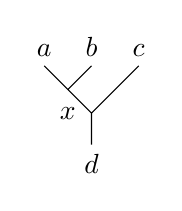
\begin{tikzpicture}[baseline=0]
  \draw
    (0,0)      -- (-0.6,0.6) node [above] {$a$}
    (-0.3,0.3) -- (0,0.6)    node [above] {$b$}
    (0,0)      -- (0.6,0.6)  node [above] {$c$}
    (0,0)      -- (0,-0.4)   node [below] {$d$}
    (-0.3,0) node {$x$};
\end{tikzpicture}

  \in \bigoplus_x V^{ab}_x \otimes V^{xc}_d \simeq V^{abc}_d, \quad
  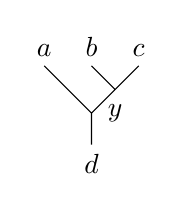
\begin{tikzpicture}[baseline=0]
  \draw
    (0,0)     -- (-0.6,0.6) node [above] {$a$}
    (0.3,0.3) -- (0,0.6)    node [above] {$b$}
    (0,0)     -- (0.6,0.6)  node [above] {$c$}
    (0,0)     -- (0,-0.4)   node [below] {$d$}
    (0.3,0) node {$y$};
\end{tikzpicture}

  \in \bigoplus_x V^{ay}_d \otimes V^{bc}_y \simeq V^{abc}_d.
\end{equation}
联系这两组基的变换称为 \emph{$F$ 移动} ($F$-move):
\begin{equation}
  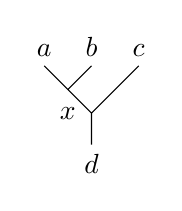
\begin{tikzpicture}[baseline=0]
  \draw
    (0,0)      -- (-0.6,0.6) node [above] {$a$}
    (-0.3,0.3) -- (0,0.6)    node [above] {$b$}
    (0,0)      -- (0.6,0.6)  node [above] {$c$}
    (0,0)      -- (0,-0.4)   node [below] {$d$}
    (-0.3,0) node {$x$};
\end{tikzpicture}

  = \sum_y \, \bigl[ F^{abc}_d \bigr]_{xy}
  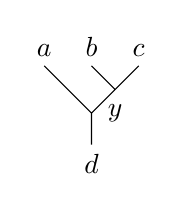
\begin{tikzpicture}[baseline=0]
  \draw
    (0,0)     -- (-0.6,0.6) node [above] {$a$}
    (0.3,0.3) -- (0,0.6)    node [above] {$b$}
    (0,0)     -- (0.6,0.6)  node [above] {$c$}
    (0,0)     -- (0,-0.4)   node [below] {$d$}
    (0.3,0) node {$y$};
\end{tikzpicture}
.
\end{equation}
式中的系数 $[F^{abc}_d]_{xy}$ 称为 \emph{$F$ 符号} ($F$-symbol),它一共有 6 个指标。

一个融合范畴可由以下几组数据完全确定:

\begin{itemize}
  \item 简单对象的集合 $\{a,b,c,\ldots\}$;
  \item 融合系数 $N_{ab}^c$ 或者对应的融合规则;
  \item $F$ 符号 $[F^{abc}_d]_{xy}$。
\end{itemize}

\section{拓扑序}

\section{弦网模型}
